\chapter{Analyse des résultats}
\par Dans cette partie nous allons analyser les résultats de chacun des algorithmes.
\section{Résultats}
\subsection{Régression logistique}
\begin{figure}[H]
    \centering
    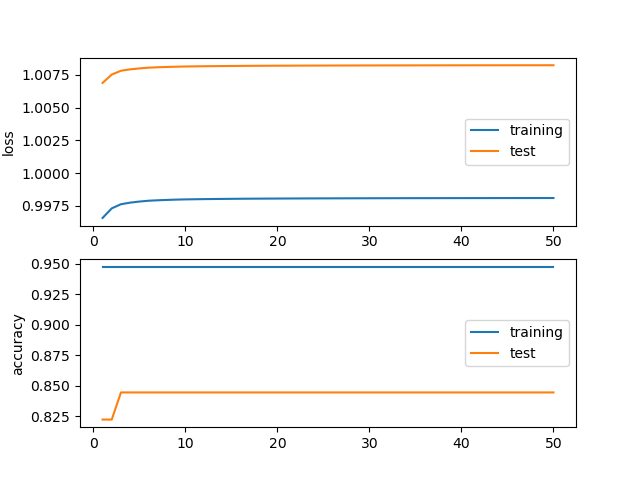
\includegraphics[width=17cm, height=10cm, keepaspectratio]{logistique_plot.png}
    \caption{Figure diagrames "accuracy" et "loss" pour la régression logistique }
    \label{Figure diagrames "accuracy" et "loss" pour la régression logistique  }
\end{figure}
\par Pour "lr" entre 0.0001 et 0.001, et pour "l2reg" entre 0.1 et 10, les meilleurs valeurs pour les hyper-paramètres "lr" et "l2reg" sont ceux affichés dans la figure ci-dessous
\begin{figure}[H]
    \centering
    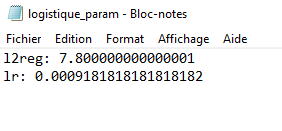
\includegraphics{logistique_param.PNG}
    \caption{Figure parametres de régression logistique}
    \label{Figure parametres de régression logistique }
\end{figure}
\subsection{SVM}
\par Les erreurs et les précisions d'entrainement et de test:
\begin{figure}[H]
    \centering
    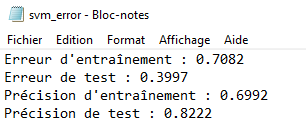
\includegraphics{svm.png}
    \caption{Figure SVM-error }
    \label{Figure fichier svm-error }
\end{figure}
\subsection{Réseaux de neuronnes}
\begin{figure}[H]
    \centering
    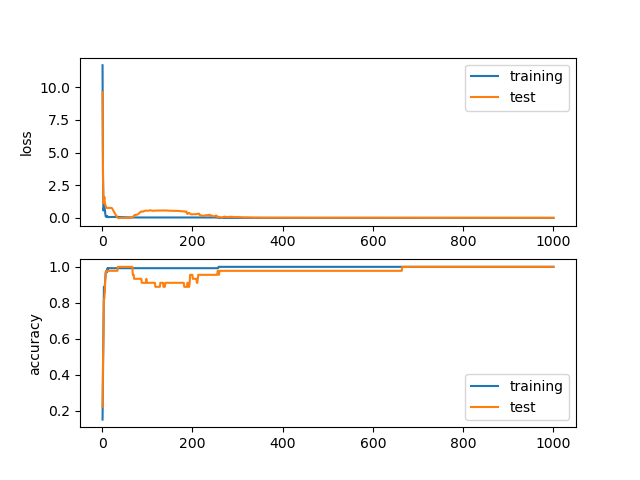
\includegraphics[width=17cm, height=10cm, keepaspectratio]{rn_plot2.png}
    \caption{Figure diagrames "accuracy" et "loss" pour réseau de neuronne a une couche cachée }
    \label{Figure diagrames "accuracy" et "loss" pour réseau de neuronne a une couche cachée }
\end{figure}  
\begin{figure}[H]
    \centering
    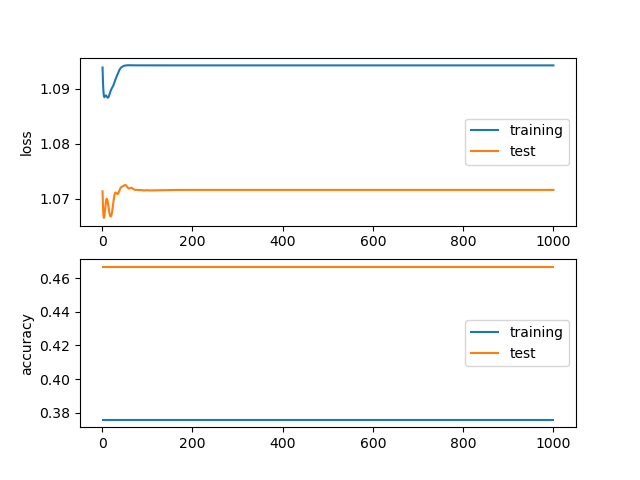
\includegraphics[width=17cm, height=10cm, keepaspectratio]{rn_plot.png}
    \caption{Figure diagrames "accuracy" et "loss" pour réseau de neuronne a deux couches cachées }
    \label{Figure diagrames "accuracy" et "loss" pour réseau de neuronne a deux couches cachées }
\end{figure}   
\par Pour "lr" entre 0.01 et 1, et pour "l2reg" entre 0.1 et 10, et pour "mu" entre 0 et 1, les meilleurs valeurs pour les hyper-paramètres "lr", "l2reg" et "mu" sont ceux affichés dans les deux figures ci-dessous
\begin{figure}[H]
    \centering
    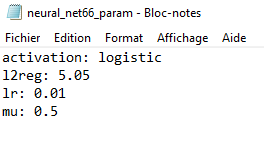
\includegraphics{rn_param_logistic.PNG}
    \caption{Figure paramètres pour réseau de neurones à deux couches cachées}
    \label{paramètres pour une fonction d'activation logistique }
\end{figure}
\begin{figure}[H]
    \centering
    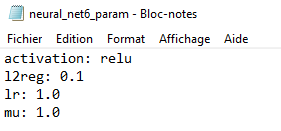
\includegraphics{rm_param_relu.PNG}
    \caption{Figure paramètres pour réseau de neurones à une couche cachée}
    \label{paramètres pour une fonction d'activation RELU }
\end{figure}
\subsection{Bagging}
\begin{figure}[H]
    \centering
    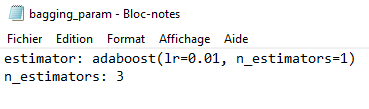
\includegraphics{bagging_param.PNG}
    \caption{Figure bagging-param }
    \label{Figure fichier bagging-param }
\end{figure}
\par Les précisions d'entrainement et de test:
\begin{figure}[H]
    \centering
    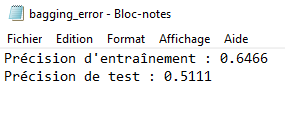
\includegraphics{bagging.PNG}
    \caption{Figure bagging-error }
    \label{Figure fichier bagging-error }
\end{figure}
\subsection{AdaBoost} 
\par Pour "lr" entre 0.01 et 1, et pour "n-estimators" entre 1 et 101, les meilleurs valeurs pour les hyper-paramètres "lr" et "n-estimator" sont ceux affichés dans la figure ci-dessous
\begin{figure}[H]
    \centering
    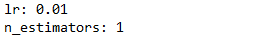
\includegraphics{adaboost_param.PNG}
    \caption{Figure adaboost-param }
    \label{Figure fichier adaboost-param }
\end{figure}
\par Les précisions d'entrainement et de test:
\begin{figure}[H]
    \centering
    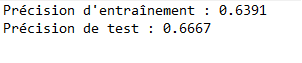
\includegraphics{adaboost.PNG}
    \caption{Figure adaboost-error }
    \label{Figure fichier adaboost-error }
\end{figure}

\section{Analyse}
\par En analysant les précisions d'entrainement et test, on constate que les algorithmes Bagging et Adaboost se sont avérés peu efficaces.
\par D'après les deux graphiques correpondants à la classification par réseau de neurones, on constate que le réseau ayant deux couches cachées ne fonctionne pas alors que  celui ayant un seule couche cachée converge rapidement vers la solution optimale.
\par La classification par régression logistique converge aussi rapidement vers la solution optimale. Ceci suggère que les données soient linéairement séparables.
\par Le réseau de neurones à une couche caché semble avoir une erreur moindre et une plus grande précision que la régression logistique. Toutefois, il lui faut un plus
grand nombre d'itérations pour
converger vers la solution optimales. La régression logistique converge plus rapidement. L'algorithme SVM avec un noyau rbf a aussi obtenu de bon résultats et, de plus, 
il est très facile à mettre en oeuvre, car il ne nécessite pas d'hyperparamètres.

